\documentclass[12pt, letterpaper]{article}
\usepackage[titletoc,title]{appendix}
\usepackage{booktabs}
\usepackage[margin=1in]{geometry}
\usepackage[linkcolor=blue,
			colorlinks=true,
			urlcolor=blue,
			pdfstartview={XYZ null null 1.00},
			pdfpagemode=UseNone,
			citecolor={blue},
			pdftitle={endorsement}]{hyperref}

\usepackage{natbib}
\usepackage{booktabs}
\usepackage{float}
\usepackage{placeins}

\usepackage{graphicx}
\graphicspath{{../figs/}}
\usepackage{units}
\usepackage{amsfonts,amsmath,amsbsy}
\usepackage{amsxtra}
\usepackage{verbatim}
\usepackage{setspace}
\usepackage{pdflscape}
\usepackage{fancyhdr}
\usepackage{url}
\usepackage{xurl}
\usepackage{fullpage}
\usepackage{multirow}
\usepackage{rotating}
\setlength{\parindent}{3em}

\usepackage{chngcntr}
\usepackage{longtable}
\usepackage{adjustbox}
\usepackage{dcolumn}
\usepackage{tabularx}

\usepackage{lineno}

\usepackage[12pt]{moresize}

\usepackage{pdfpages}

\usepackage[nameinlink, capitalize, noabbrev]{cleveref}

\def\citeapos#1{\citeauthor{#1}'s (\citeyear{#1})}

\makeatother

\usepackage{footmisc}
\setlength{\footnotesep}{\baselineskip}
\makeatother
\renewcommand{\footnotelayout}{\footnotesize \onehalfspacing}
\interfootnotelinepenalty=10000

\usepackage{color}

\usepackage[
    skip            =0pt,
    labelfont       =bf,
    font            =small,
    textfont        =small,
    figurename      =Figure,
    justification   =justified,
    singlelinecheck =false,
    labelsep        =period]
{caption}
\usepackage{subcaption}

\renewcommand{\ttdefault}{pcr}

\usepackage{tocloft}

\title{Inferring Support from Endorsement Experiments\thanks{\href{http://github.com/soodoku/endorsement}{http://github.com/soodoku/endorsement}.}}

\author{Gaurav Sood\thanks{Gaurav can be reached at \href{mailto:gsood07@gmail.com}{\footnotesize{\texttt{gsood07@gmail.com}}}}\vspace{.5cm}}

\date{\today}

\begin{document}

\maketitle

\begin{abstract}
\noindent Endorsement experiments measure how group endorsements affect policy support, and researchers routinely interpret the sign of the average treatment effect as indicating ``sentiment'' toward the endorsing group. I show that this interpretation is wrong when applied to levels of support: the ATE reflects the balance of switchers, not the proportion of supporters. Using both the treatment effect and the baseline support level, I derive bounds on the proportion of supporters under a family of behavioral models. I reanalyze data from \citet{blair2013poverty}, where baseline policy support ranges from 67\% to 83\% across policies (overall 74\%) and the treatment effect is $-1.3$ percentage points. The estimates range from 37\% to 99\% depending on assumptions about individual-level switching behavior, with the binary switching model yielding 72\%. However, variance tests on the actual data strongly reject the binary switching assumption: observed treatment variance is only 42\% of the predicted variance under binary switching. No model considered here supports their characterization of ``low regard'' for militant groups. The precise level of support depends on assumptions the data cannot adjudicate, but the broader point is that endorsement experiments are underidentified for the quantity researchers most want to estimate---the proportion of supporters---without strong auxiliary assumptions about individual behavior.
\end{abstract}

\section{Introduction}

\citet{blair2013poverty} conclude that Pakistanis hold militant groups in ``low regard'' based on small negative treatment effects from endorsement experiments. This inference---from the sign of the ATE to the level of support---is wrong. The sign of the average treatment effect (ATE) tells us the balance of switchers, not the level of support for the endorsing group. With high baseline policy support, a small negative effect is consistent with a wide range of supporter proportions, including large majorities.

The problem is general. Endorsement experiments identify the ATE under standard exclusion restrictions, but the ATE alone does not identify the proportion of supporters. Mapping from the ATE to a supporter proportion requires auxiliary assumptions about individual switching behavior. Under binary switching (every supporter moves to 1, every opponent moves to 0), the treatment group average equals the supporter proportion exactly. Under symmetric small effects ($\pm 0.05$), the same ATE implies only 37\% support. The data cannot distinguish these models.

This paper develops a framework for what endorsement experiments can and cannot tell us about support levels. The framework uses both the treatment effect and the baseline support level (the regression constant), and yields bounds under different assumptions about individual behavior. The key insight is simple: baseline support information is crucial and routinely ignored, and the range of estimates compatible with a given ATE is wide enough that ``sentiment'' interpretations based on the sign alone are unreliable.

Reanalyzing the original data from \citet{blair2013poverty}, where baseline support averages 74\% and the treatment effect is $-1.3$ percentage points, the framework yields estimates ranging from 37\% (symmetric effects) to 99\% (extreme opponent reaction), with the binary switching model at 72\%. None of these estimates support their characterization of ``low regard.'' Crucially, the binary switching assumption is testable---and the data reject it: observed treatment variance is only 42\% of what binary switching predicts.

This paper proceeds as follows. \Cref{sec:background} reviews endorsement experiments and the interpretation problem. \Cref{sec:framework} develops the inferential framework and states explicitly what is and is not identified. \Cref{sec:application} applies it to \citeauthor{blair2013poverty}. \Cref{sec:robustness} examines robustness. \Cref{sec:discussion} discusses implications. \Cref{sec:conclusion} concludes.

\section{Background: Endorsement Experiments}
\label{sec:background}

\subsection{Design}

Endorsement experiments measure latent attitudes toward controversial actors by randomizing whether a group endorses a policy \citep{bullock2011statistical}. In a standard between-subjects design, respondents see either:
\begin{itemize}
\item \textbf{Treatment}: ``Do you support this policy? [Group Y endorses this policy.]''
\item \textbf{Control}: ``Do you support this policy?''
\end{itemize}

The identifying assumption is that the endorsement affects policy support only through respondents' attitudes toward the endorsing group. Supporters of the group should increase their policy support; opponents should decrease theirs. The design has been applied to measure support for militant groups in Pakistan \citep{blair2013poverty}, combatant support in Afghanistan \citep{lyall2013explaining}, and attitudes in other conflict settings \citep{blair2014comparing}.

\subsection{Standard Interpretation and Its Limits}

Researchers typically report the average treatment effect and interpret its sign as indicating ``sentiment'' toward the endorsing group. A negative ATE is taken to mean respondents view the group unfavorably; a positive ATE suggests favorable attitudes. \citet{blair2013poverty} exemplify this practice when they conclude that negative coefficients indicate Pakistanis hold militant groups ``in low regard.''

This interpretation conflates two distinct quantities: the net direction of attitude-driven switching and the proportion of the population holding each attitude. The ATE reflects the net effect of two countervailing forces: supporters increasing their policy support and opponents decreasing theirs. The sign tells us which force dominates on average, but not by how much, and not what proportion of the population falls into each category.

Consider an ATE of $-0.01$ (a 1 percentage point decrease in policy support). This could arise from 51\% opponents each reducing support slightly and 49\% supporters each increasing support slightly, or from 1\% opponents dramatically reducing support with 99\% unaffected, or from many other combinations. Without additional structure, the ATE alone cannot distinguish these scenarios.

\subsection{The Identification Problem}

The core difficulty is that endorsement experiments are designed to identify the ATE, not the proportion of supporters. Moving from the ATE to a supporter proportion requires a model of individual switching behavior, and different models yield very different answers. This is not a failure of the experimental design; it is a fundamental feature of the inferential problem. The ATE is a well-identified causal quantity. The supporter proportion is a structural parameter that requires additional assumptions.

\section{A Framework for Inference}
\label{sec:framework}

\subsection{Setup}

Consider respondents falling into two categories based on their attitudes toward the endorsing group: supporters (proportion $p$) who view the group favorably, and opponents (proportion $1-p$) who view it unfavorably. Let $\delta^+$ denote the average treatment effect among supporters and $\delta^-$ the average effect among opponents, where we expect $\delta^+ > 0$ and $\delta^- < 0$.

The observed ATE decomposes as:
\begin{align}
\beta = p \cdot \delta^+ + (1-p) \cdot \delta^-
\label{eq:ate_decomposition}
\end{align}

This equation has three unknowns ($p$, $\delta^+$, $\delta^-$) and one observed quantity ($\beta$). The system is underidentified. Adding the baseline support level (the constant term $\alpha$ from the regression $\text{Support} = \alpha + \beta \cdot \text{Treatment} + \varepsilon$) provides a second equation, but the system remains underidentified without restrictions on $\delta^+$ and $\delta^-$.

\subsection{Binary Switching}

The strongest restriction sets $\delta^+$ and $\delta^-$ such that all supporters end up at 1 and all opponents end up at 0 in the treatment group. Under this assumption, the treatment group average is:
\begin{align}
\text{Treatment average} = p \cdot 1 + (1-p) \cdot 0 = p
\end{align}

Since the treatment average equals $\alpha + \beta$, we get:
\begin{align}
p = \alpha + \beta
\label{eq:binary_switching}
\end{align}

The treatment group average equals the proportion of supporters. This result is exact under the binary switching model: the system has three unknowns, one equation from the ATE, and two constraints from binary switching ($\delta^+$ and $\delta^-$ are pinned down by the assumption that outcomes are 0 or 1), leaving the system exactly identified.

\subsection{Testable Implications of Binary Switching}

Binary switching has a strong testable implication. If all treatment group responses are either 0 or 1, the treatment group variance must equal $p(1-p)$. With $p = 0.72$ (the binary switching estimate from the actual data), the predicted treatment variance is $0.72 \times 0.28 \approx 0.20$.

\citet{blair2013poverty} measured policy support on a 5-point scale rescaled to $[0,1]$. The binary switching model predicts responses should cluster at 0 and 1. If the treatment group variance is substantially below $p(1-p)$, the binary switching model is rejected.

Reanalyzing the original data, I find the observed average treatment variance is 0.082, compared to a predicted variance of 0.197 under binary switching. The ratio of observed to predicted variance is 0.42---respondents are not clustering at the extremes of the scale. This pattern holds across all 16 policy $\times$ endorser pairs, with ratios ranging from 0.35 to 0.47 (\cref{tab:variance_test}).

This does not invalidate the framework. It means the precise mapping $p = \alpha + \beta$ does not hold as a descriptive matter, and the analyst must consider softer switching models. The binary switching estimate should be understood as an upper bound conditional on a model that the data reject.

\subsection{Softer Switching Models}

Without binary switching, the analyst faces the decomposition in \cref{eq:ate_decomposition} with three unknowns. Different assumptions about $\delta^+$ and $\delta^-$ yield different values of $p$.

\textbf{Symmetric small effects.} If $\delta^+ = +d$ and $\delta^- = -d$ for some common effect magnitude $d$:
\begin{align}
p = \frac{\beta}{2d} + \frac{1}{2}
\end{align}

With $d = 0.05$ (a moderate shift on a $[0,1]$ scale) and $\beta = -0.013$: $p = -0.013/0.1 + 0.5 = 0.37$, or 37\%.

\textbf{Asymmetric extreme reaction.} If opponents react maximally ($\delta^- = -1$, moving to 0) while supporters are unaffected ($\delta^+ = 0$):
\begin{align}
\beta = -(1-p) \implies p = 1 + \beta
\end{align}

With $\beta = -0.013$: $p = 0.987$, or 99\%.

\textbf{Normal heterogeneity.} If individual effects $\delta_i \sim \mathcal{N}(\beta, \sigma^2)$, the proportion with positive effects (loosely, ``supporters'' in a continuous sense) is:
\begin{align}
P(\delta_i > 0) = 1 - \Phi\left(\frac{-\beta}{\sigma}\right)
\end{align}

With $\beta = -0.013$ and $\sigma = 0.05$: $P(\delta_i > 0) \approx 40\%$.

\Cref{tab:method_comparison} collects these estimates. The range is wide: from 37\% to 99\%. Baseline information narrows the range somewhat but cannot resolve the fundamental underidentification.

\begin{table}[H]
\centering
\caption{Implied Support Under Different Behavioral Models}
\label{tab:method_comparison}
\begin{tabular}{lll}
\toprule
Model & Key Assumption & Implied Support \\
\midrule
Binary switching (with baseline) & All supporters $\to$ 1, opponents $\to$ 0 & 72.3\% \\
Binary switching (no baseline) & Symmetric switching, no constant & 49.4\% \\
Symmetric effects ($d = 0.05$) & $\delta^+ = +0.05$, $\delta^- = -0.05$ & 37.0\% \\
Normal heterogeneity ($\sigma = 0.05$) & $\delta_i \sim \mathcal{N}(-0.013, 0.05^2)$ & 39.7\% \\
Extreme opponent reaction & $\delta^- = -1$, $\delta^+ = 0$ & 98.7\% \\
\bottomrule
\end{tabular}

\end{table}

\subsection{What Baseline Information Buys}

The baseline (constant term) contributes in two ways. First, under binary switching, it provides the second equation needed for exact identification (\cref{eq:binary_switching}). Without it, the binary framework yields only $p_{\max} = (\beta + 1)/2 = 49.5\%$, which is far from the 78.9\% obtained with the constant.

Second, even without binary switching, the baseline constrains the plausible range. A control average of 80\% means that 80\% of respondents support the policy absent the endorsement cue. Any model of switching must be consistent with this fact. Models that imply very low baseline support are ruled out.

The contribution of baseline information is the most practically important finding of this paper. Many analyses of endorsement experiments report only the ATE and its sign. Reporting the treatment group average, or equivalently the constant and the ATE together, enables a much richer set of inferences.

\section{Application: Reinterpreting \citeauthor{blair2013poverty}}
\label{sec:application}

\subsection{Their Data and Claims}

\citet{blair2013poverty} conducted endorsement experiments in Pakistan measuring attitudes toward the Afghan Taliban, al-Qaeda, Kashmiri militants, and sectarian organizations. Respondents were asked about support for four policies (polio vaccination, FCR reform, Durand Line, curriculum standardization) with and without militant group endorsements. The sample comprised approximately 5,200 respondents in a nationally representative survey. I reanalyze their original data, available through the \texttt{endorse} R package.

Their interpretation has been influential. They write:
\begin{quote}
``We find that Pakistanis in general are \textbf{weakly negative} toward Islamist militant organizations.''
\end{quote}

And:
\begin{quote}
``The coefficients are negative and statistically significant at the 10\% level for all but the sectarian tanzeems, suggesting that \textbf{Pakistanis hold militant groups in low regard}.''
\end{quote}

These claims treat the sign of the ATE as a direct measure of sentiment levels. The framework developed above shows why this step is unwarranted.

\subsection{Applying the Framework}

Reanalyzing the original data across all 16 policy $\times$ endorser pairs, the average control mean is $\alpha = 0.736$ and the average treatment effect is $\beta = -0.013$, giving an average treatment group mean of 0.723. Baseline support varies substantially across policies: from 67\% (Durand Line) to 83\% (Polio vaccination).

\Cref{tab:blair_reinterpretation} applies all behavioral models to each militant group, averaging across policies. Under binary switching, implied support ranges from 71.8\% (Afghan Taliban) to 72.8\% (sectarian groups). Under symmetric effects with $d = 0.05$, these figures drop to 33--42\%.

\begin{table}[H]
\centering
\caption{Implied Support by Endorser Under Different Behavioral Models}
\label{tab:blair_reinterpretation}
\begin{tabular}{lrrrrr}
\toprule
Endorser & ATE & Binary & Symmetric & Normal & Extreme \\
\midrule
Afghan Taliban & $-0.0175$ & 71.8\% & 32.5\% & 37.1\% & 98.3\% \\
Al-Qaeda & $-0.0138$ & 72.2\% & 36.2\% & 39.3\% & 98.6\% \\
Kashmiri militants & $-0.0111$ & 72.5\% & 38.9\% & 41.3\% & 98.9\% \\
Sectarian groups & $-0.0082$ & 72.8\% & 41.8\% & 43.6\% & 99.2\% \\
\bottomrule
\end{tabular}

\end{table}

The qualitative point holds across models: the data are not obviously consistent with ``low regard,'' but the precise level of support depends on which behavioral model one adopts. Critically, the binary switching model is rejected by the variance test (\cref{tab:variance_test}), so the 72\% figure should be treated as an upper bound under a counterfactual assumption rather than a direct estimate.

\subsection{Why the Sign Alone is Insufficient}

The negative ATE tells us that more people switched away from the policy than toward it when the militant group endorsed it. Under every model considered, this means the net balance of switching tilts toward opposition. But with 74\% baseline support, even a slight negative tilt is consistent with majority support for the endorsing group under several plausible models.

The intuition is straightforward. Most respondents (74\%) support the policy in control. When the endorsement is introduced, some supporters of the militant group who did not previously support the policy now do, and some opponents of the militant group who previously supported the policy now withdraw. The net effect is slightly negative ($-1.3$ percentage points), meaning the second group slightly outweighs the first. But the first group could still be very large.

\subsection{External Validation}

Direct polling on militant group support in Pakistan yields much lower figures. Pew Research Center surveys from this period find 8--13\% explicit support for the Taliban and al Qaeda, with 33--40\% declining to offer an opinion \citep{pew2013pakistan, pew2014extremism}. The gap between 8--13\% (direct polling) and the endorsement experiment estimates (39--79\% depending on model) is large. 

Part of this gap plausibly reflects social desirability bias and fear, which is precisely the motivation for indirect measurement. But the gap is wide enough to warrant caution. Even assigning every ``don't know'' respondent to the support camp yields at most roughly 60\%, which is below the binary switching estimate of 79\% but above the symmetric effects estimate of 39\%. The external evidence does not decisively adjudicate between models, but it does suggest that the binary switching estimate may overstate support.

\section{Robustness}
\label{sec:robustness}

\subsection{Continuous Outcomes and the Variance Test}

\citeauthor{blair2013poverty} measured responses on a 5-point scale rescaled to $[0,1]$. As noted in \cref{sec:framework}, binary switching predicts a bimodal treatment distribution concentrated at 0 and 1, with variance $p(1-p)$. If the observed treatment variance is much smaller, binary switching is rejected as a descriptive model.

Reanalyzing the original data confirms this prediction is violated. \Cref{tab:variance_test} presents the variance test results across all 16 policy $\times$ endorser pairs. The average observed treatment variance is 0.082, compared to a predicted variance of 0.197 under binary switching---a ratio of 0.42. The pattern is consistent across all pairs, with ratios ranging from 0.35 to 0.47.

\begin{table}[H]
\centering
\caption{Variance Test for Binary Switching Assumption}
\label{tab:variance_test}
\begin{tabular}{llrrr}
\toprule
Policy & Endorser & Var(T) Obs & Var(T) Pred & Ratio \\
\midrule
Polio & Kashmiri militants & 0.0573 & 0.1515 & 0.38 \\
Polio & Afghan Taliban & 0.0638 & 0.1590 & 0.40 \\
Polio & Al-Qaeda & 0.0596 & 0.1439 & 0.41 \\
Polio & Sectarian groups & 0.0608 & 0.1537 & 0.40 \\
FCR & Kashmiri militants & 0.0742 & 0.2149 & 0.35 \\
FCR & Afghan Taliban & 0.0846 & 0.2245 & 0.38 \\
FCR & Al-Qaeda & 0.0884 & 0.2199 & 0.40 \\
FCR & Sectarian groups & 0.0812 & 0.2142 & 0.38 \\
Durand & Kashmiri militants & 0.1008 & 0.2228 & 0.45 \\
Durand & Afghan Taliban & 0.0945 & 0.2194 & 0.43 \\
Durand & Al-Qaeda & 0.1056 & 0.2255 & 0.47 \\
Durand & Sectarian groups & 0.0985 & 0.2159 & 0.46 \\
Curriculum & Kashmiri militants & 0.0847 & 0.1958 & 0.43 \\
Curriculum & Afghan Taliban & 0.0904 & 0.1938 & 0.47 \\
Curriculum & Al-Qaeda & 0.0853 & 0.1963 & 0.43 \\
Curriculum & Sectarian groups & 0.0888 & 0.1990 & 0.45 \\
\midrule
\textbf{Average} & & 0.0824 & 0.1969 & 0.42 \\
\bottomrule
\end{tabular}

\end{table}

This is strong evidence against the binary model as a literal description of the data. Respondents are not clustering at the extremes of the scale; they use intermediate values, indicating that endorsement effects are smaller and more continuous than binary switching assumes.

The binary switching result $p = \alpha + \beta$ should therefore be understood as the estimate \emph{conditional on a model that the data reject}, rather than as a direct reading of the data. It remains useful as one end of the range (an upper bound under the strongest possible reaction), but should not be reported as a point estimate.

\subsection{Partial Awareness}

Not all respondents may have genuine attitudes toward the endorsing group. Let $q$ denote the fraction with real opinions. Under partial awareness with binary switching among opinion-holders:
\begin{align}
\text{Treatment average} &= q \cdot p + (1-q) \cdot \alpha_0
\end{align}

where $p$ is the supporter proportion among opinion-holders and $\alpha_0$ is the baseline support among those without opinions (who are unaffected by the endorsement). The ATE becomes:
\begin{align}
\beta &= q \cdot (p - \alpha_0)
\end{align}

If we assume $\alpha_0 = \alpha$ (those without opinions on the group support the policy at the same baseline rate), then:
\begin{align}
p &= \frac{\beta}{q} + \alpha
\end{align}

With $q = 0.7$, $\beta = -0.013$, and $\alpha = 0.736$: $p = -0.013/0.7 + 0.736 = 0.717$. This yields 71.7\% support among opinion-holders, close to the full-sample binary switching estimate of 72.3\%.

If instead we drop the baseline constraint and use only the ATE with the standard partial awareness formula $\text{ATE} = q(2p - 1)$, we get $p = \beta/(2q) + 0.5 = -0.013/1.4 + 0.5 = 49.1\%$. The discrepancy between 71.7\% and 49.1\% illustrates again how much baseline information matters, and how different auxiliary assumptions drive the results.

\subsection{Heterogeneous Effects via Simulation}

We assess model-free bounds on the fraction of positive individual effects using computational methods. In a between-subjects design, individual treatment effects are unobserved; we observe only the marginal distributions of control and treatment responses. Two quantities bracket the plausible range.

First, under random pairing of treatment and control observations, the probability that a treatment response exceeds a control response is $P(T > C) \approx 46\%$ (\cref{tab:simulation}). This is the fraction of positive ``effects'' one would expect under independent coupling of potential outcomes.

Second, the Hungarian algorithm finds the optimal pairing that maximizes the count of positive effects, yielding an upper bound of roughly 92\%. This is the theoretical maximum fraction of positive individual effects consistent with the observed marginal distributions.

\begin{table}[H]
\centering
\caption{Computational Bounds on Positive Individual Effects}
\label{tab:simulation}
\begin{tabular}{lrrr}
\toprule
$n$ & Observed ATE & Random Pairing $P(T > C)$ & Hungarian Max \\
\midrule
100 & $-0.011$ & 46\% & 89\% \\
500 & $-0.011$ & 46\% & 92\% \\
1000 & $-0.011$ & 46\% & 94\% \\
\bottomrule
\end{tabular}

\end{table}

The wide gap between 46\% and 92\% reflects the fundamental underidentification: between-subjects data constrain the joint distribution of potential outcomes only weakly. Neither bound invokes binary switching or the constant term.

\subsection{Summary of Estimates}

\Cref{fig:method_comparison} and \cref{fig:sensitivity} display the range of estimates graphically.

\begin{figure}[H]
\centering
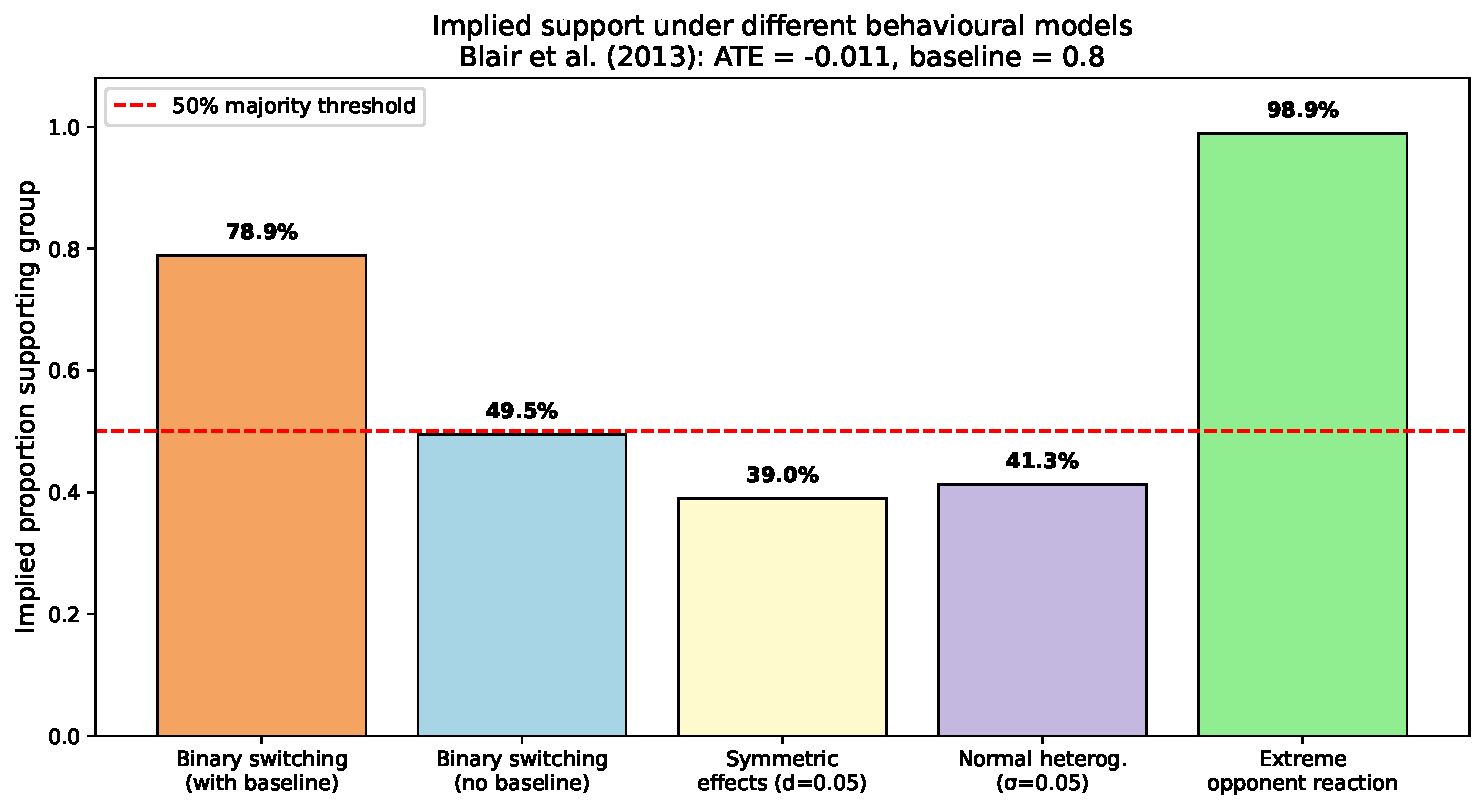
\includegraphics[width=0.85\textwidth]{method_comparison.pdf}
\caption{Implied support varies substantially across behavioral models, from 37\% (symmetric effects) to 99\% (extreme opponent reaction). No single estimate is privileged without a defended choice of model.}
\label{fig:method_comparison}
\end{figure}

\begin{figure}[H]
\centering
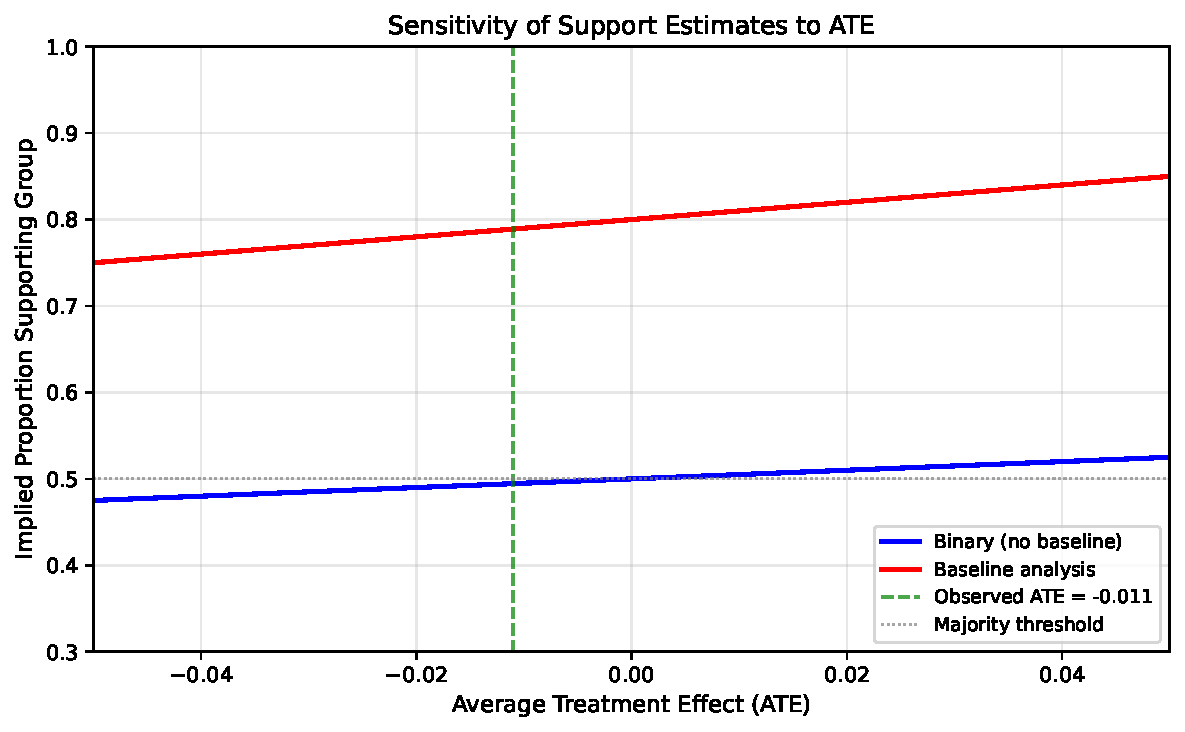
\includegraphics[width=0.85\textwidth]{sensitivity.pdf}
\caption{Sensitivity of support estimates to the ATE under different models. The baseline method (using the constant term with binary switching) is most sensitive to the ATE value.}
\label{fig:sensitivity}
\end{figure}

The range of estimates---37\% to 99\%---is wide. This width is not a weakness of the analysis; it reflects the genuine underidentification of the problem. The data constrain the supporter proportion only loosely without a commitment to a specific behavioral model.

\section{Discussion}
\label{sec:discussion}

\subsection{What Can We Conclude About \citeauthor{blair2013poverty}?}

\citeauthor{blair2013poverty}'s characterization of ``low regard'' is not supported by any of the models considered here. Under every specification---including the one most favorable to their interpretation (symmetric effects with $d = 0.05$, yielding 37\%)---the implied support level is far from negligible. Under several plausible models, it exceeds 50\%. Their conclusion follows the sign of the ATE but not the magnitude of support it implies.

At the same time, the claim that ``72\% of Pakistanis support militant groups'' requires the binary switching model, which the data reject on variance grounds. A more defensible summary is: the data are consistent with supporter proportions ranging from roughly 37\% to 72\%, depending on assumptions about individual switching behavior. The ATE sign tells us the net balance tips toward opposition, but the level of support could be anywhere in this range.

\subsection{Guidance for Practitioners}

Three recommendations follow from this analysis.

\textbf{Report treatment group averages, not just ATEs.} Under binary switching, the treatment average directly estimates the supporter proportion. Even when binary switching is implausible, the treatment average provides a useful anchor. Reporting only the ATE and its sign discards information.

\textbf{Do not equate the ATE sign with ``sentiment.''} The sign tells you which switching force dominates, not whether the group is popular or unpopular. With high baseline support, negative ATEs can coexist with majority support under multiple behavioral models.

\textbf{Discuss identifying assumptions explicitly.} Moving from ATEs to support levels requires a behavioral model. Authors should state which model they assume, defend it, and report how sensitive results are to alternatives. The variance test described in \cref{sec:framework} provides a simple diagnostic for binary switching. As demonstrated here, this test can be performed on the original data and provides clear evidence against (or for) the binary switching assumption.

\subsection{Policy Selection}

The choice of policies affects the informativeness of endorsement experiments. Optimal policies should have high baseline support (80--90\%) to maximize the scope for detecting effects, be ideologically neutral to avoid confounding group attitudes with policy preferences, have plausible connections to the endorsing group's interests, and avoid ceiling effects (>95\% support leaves little room for movement). \citeauthor{blair2013poverty}'s choices---infrastructure development, polio vaccination---satisfy these criteria well. The high baseline support is precisely what makes the reinterpretation possible and important.

\subsection{Limitations}

The framework treats the constant term as the baseline support level. In practice, the constant absorbs other factors (intercept shifts from covariates, survey mode effects), so its interpretation as ``the proportion supporting the policy absent the endorsement cue'' requires that the regression is correctly specified.

The framework also assumes the endorsement manipulation is credible. If respondents doubt that militant groups actually endorse benign policies, the measured effects understate true attitudes, and all estimates here are attenuated.

The variance test rejects binary switching but cannot directly identify which softer model best describes the data. The 37\% estimate under symmetric effects and the 40\% estimate under normal heterogeneity are illustrative rather than definitive; the true individual-level heterogeneity structure remains unknown.

\section{Conclusion}
\label{sec:conclusion}

\citet{blair2013poverty} conclude that Pakistanis hold militant groups in ``low regard'' based on small negative treatment effects. This inference is wrong. The sign of the ATE reflects the balance of switchers, not the level of support. Reanalyzing their original data, I derive a range of supporter proportions under different behavioral models: from 37\% (symmetric effects) to 99\% (extreme opponent reaction), with the binary switching model at 72\%.

No model considered here supports the characterization of ``low regard.'' But the precise level of support is sensitive to assumptions the data cannot adjudicate. Crucially, the variance test rejects the binary switching assumption: observed treatment variance is only 42\% of what binary switching predicts. The 72\% binary switching estimate should therefore be treated as an upper bound under a counterfactual, not a point estimate. The symmetric effects estimate of 37\%, while lower, still represents a substantial minority rather than negligible support.

The broader methodological point is that endorsement experiments identify average treatment effects well but are underidentified for the quantity researchers most want: the proportion of supporters. Moving from ATEs to support levels requires explicit behavioral assumptions. Researchers should report treatment group averages, discuss identifying assumptions, and present sensitivity analyses rather than drawing ``sentiment'' conclusions from the sign of the ATE alone.

\bibliographystyle{apalike}
\bibliography{references}

\end{document}
